\documentclass[12pt,letterpaper]{ctexart}
\usepackage{fullpage}
\usepackage[top=2cm, bottom=4.5cm, left=2.5cm, right=2.5cm]{geometry}
\usepackage{amsmath,amsthm,amsfonts,amssymb,amscd}
\usepackage{lastpage}
\usepackage{enumerate}
\usepackage[binary-units=true]{siunitx}
\usepackage{fancyhdr}
\usepackage{mathrsfs}
\usepackage{xcolor}
\usepackage{graphicx} %插入图片的宏包
\usepackage{float} %设置图片浮动位置的宏包
\usepackage{subfigure} %插入多图时用子图显示的宏包
\usepackage{listings}
\usepackage{afterpage}
\usepackage{hyperref}
\hypersetup{
    colorlinks=true,
    linkcolor=blue,
    filecolor=magenta,
    urlcolor=cyan,
}

\newcommand\blankpage{%
  \null
  \thispagestyle{empty}%
  \addtocounter{page}{-1}%
  \newpage
}


\hypersetup{%
  colorlinks=true,
  linkcolor=blue,
  linkbordercolor={0 0 1}
}

\renewcommand\lstlistingname{Algorithm}
\renewcommand\lstlistlistingname{Algorithms}
\def\lstlistingautorefname{Alg.}

\lstdefinestyle{Python}{
    language        = Python,
    frame           = lines,
    basicstyle      = \footnotesize,
    keywordstyle    = \color{blue},
    stringstyle     = \color{green},
    commentstyle    = \color{red}\ttfamily
}

\setlength{\parindent}{0.0in}
\setlength{\parskip}{0.05in}

% Edit these as appropriate
\newcommand\course{CS305}
\newcommand\hwnumber{6}                  % <-- homework number
\newcommand\NetIDa{11711918}           % <-- NetID of person #1
\newcommand\NetIDb{吴烨昌}           % <-- NetID of person #2 (Comment this line out for problem sets)

\pagestyle{fancyplain}
\headheight 35pt
\lhead{\NetIDa}
\lhead{\NetIDa\\\NetIDb}                 % <-- Comment this line out for problem sets (make sure you are person #1)
\chead{\textbf{\Large Assignment \hwnumber}}
\rhead{\course \\ \today}
\lfoot{}
\cfoot{}
\rfoot{\small\thepage}
\headsep 1.5em

\begin{document}

\section*{Problem 1}

{\bf Description}

Open ``Network'' view in ``developer tools'' of browse(such as chrome) to observe
\begin{itemize}
  \item Is there any `mpd' files, What’s its name, what is the description of `mpd' in mime
  \item Is there any `m4s' files, what’s its related rate, will the files’ `rate' change along with the changing of network condition(especially the bandwidth)
\end{itemize}


{\bf Solution}

Open url \href{http://reference.dashif.org/dash.js/nightly/samples/dash-if-reference-player}{http://reference.dashif.org/dash.js/nightly/samples/dash-if-reference-player},
and watch ``Network'' tab in ``DevTools''.


\begin{itemize}
  \item Is there any `mpd' files, What’s its name, what is the description of `mpd' in mime
  \begin{figure}[H]
    \centering
    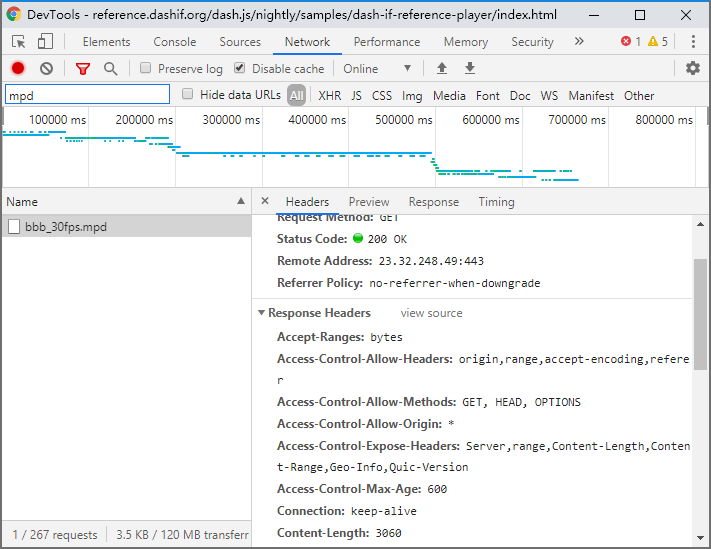
\includegraphics[width=0.8\linewidth]{assets/6.1_mpd.png}
    \caption{Command to send DNS query by TCP}
    \label{fig:cmd_tcp}
  \end{figure}
  \item Is there any `m4s' files, what’s its related rate, will the files’ `rate' change along with the changing of network condition(especially the bandwidth)


  \begin{figure}[H]
    \centering
    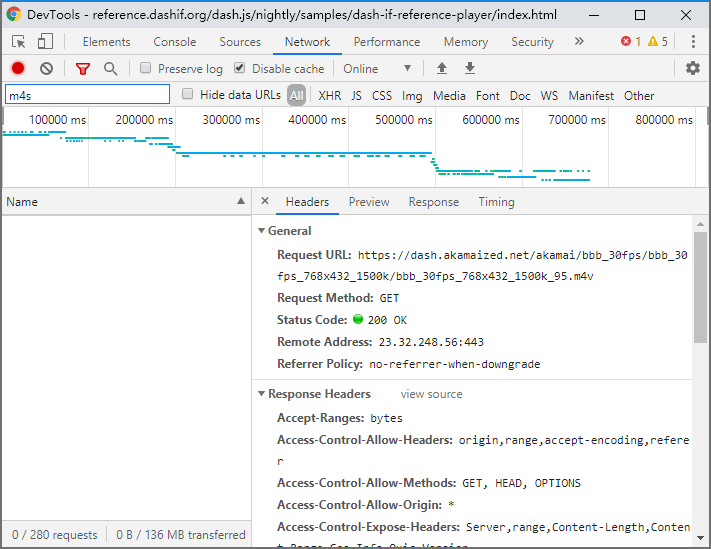
\includegraphics[width=0.8\linewidth]{assets/6.1_m4s.png}
    \caption{Command to send DNS query by TCP}
    \label{fig:cmd_tcp}
  \end{figure}

  \begin{figure}[H]
    \centering
    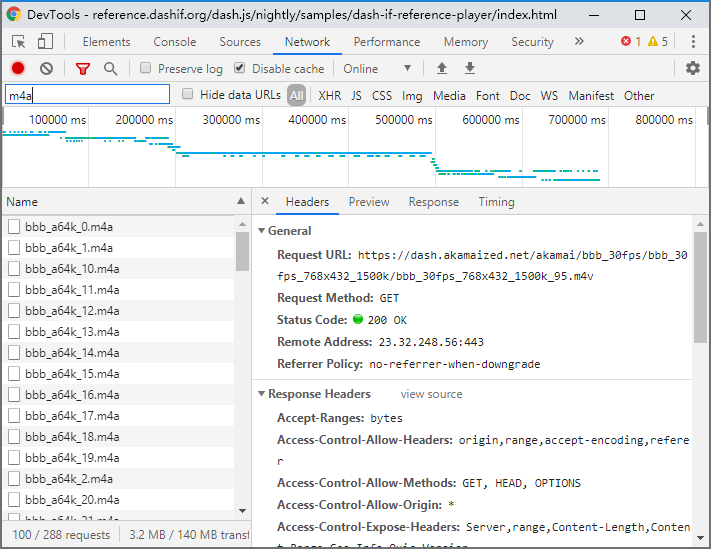
\includegraphics[width=0.8\linewidth]{assets/6.1_m4a.png}
    \caption{Command to send DNS query by TCP}
    \label{fig:cmd_tcp}
  \end{figure}

  \begin{figure}[H]
    \centering
    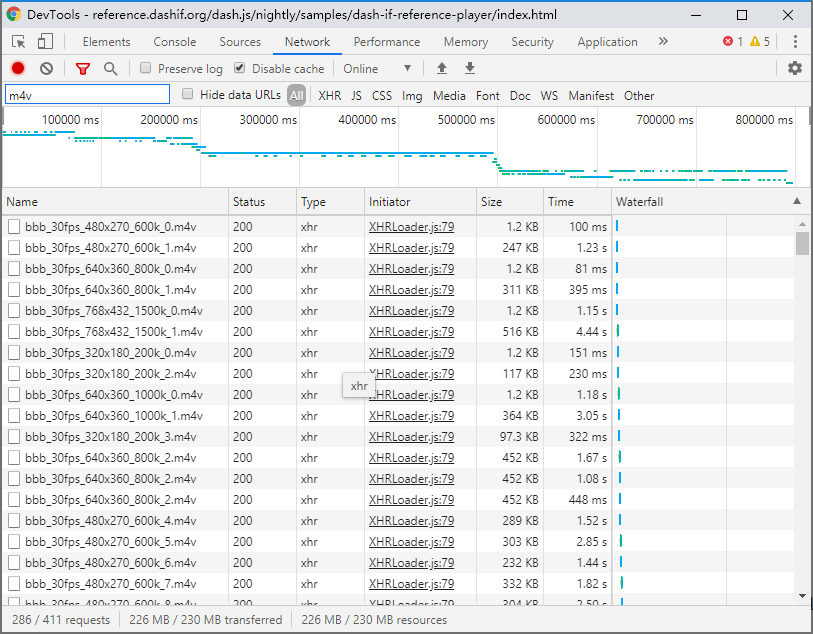
\includegraphics[width=0.8\linewidth]{assets/6.1_m4v.png}
    \caption{Command to send DNS query by TCP}
    \label{fig:cmd_tcp}
  \end{figure}
\end{itemize}


\newpage

\section*{Problem 2}

{\bf Description}

\begin{itemize}
  \item Make the query by using query method of ``dns resolver''(a python package)
  \begin{itemize}
    \item To query the type A value of \href{www.sina.com.cn}{www.sina.com.cn} based on TCP and UDP stream respectively
  \end{itemize}
  \item capture the related TCP stream and UDP stream using Wireshark
  \begin{itemize}
    \item Screenshot on this two commands.

    what's the default transport lay protocol while invoke DNS query
    \item Screenshot on the TCP stream of query by TCP.

    how many TCP packets are captured in this stream, Which port is used?
    \item Screenshot on the UDP stream of query by UDP

    how many UDP packets are captured in this stream, Which port is used?
    \item Is there any difference on DNS query and response message while using TCP and UDP respectively
  \end{itemize}
\end{itemize}


{\bf Solution}

\begin{itemize}
  \item Capture the related TCP stream and UDP stream using Wireshark
  \begin{itemize}
    \item Screenshot on this two commands.
    \begin{figure}[H]
      \centering
      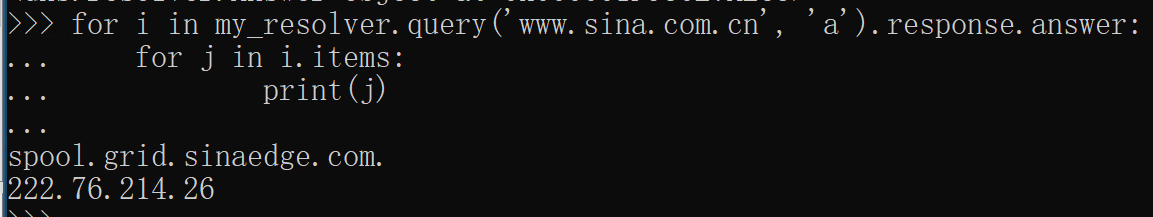
\includegraphics[width=0.8\linewidth]{assets/cmd_udp.png}
      \caption{Command to send DNS query by UDP}
      \label{fig:cmd_udp}
    \end{figure}

    The default transport lay protocol while invoke DNS query is {\bf UDP}.
    \item Screenshot on the TCP stream of query by TCP.

    \begin{figure}[H]
      \centering
      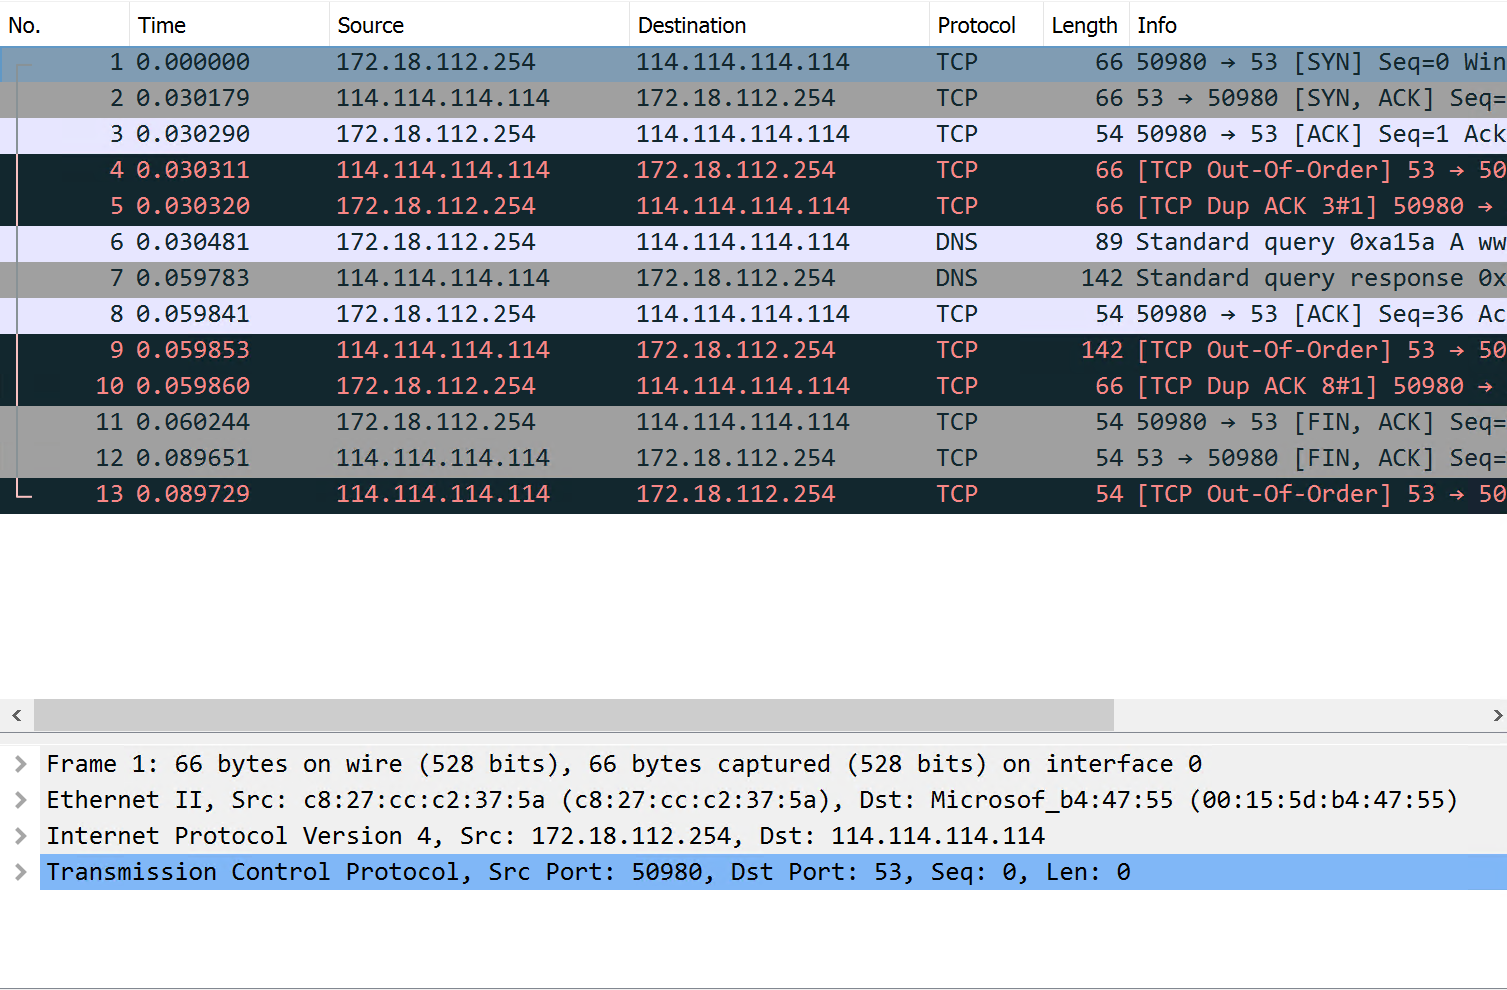
\includegraphics[width=0.8\linewidth]{assets/pic_tcp.png}
      \caption{TCP stream of query by TCP.}
      \label{fig:pic_tcp}
    \end{figure}
    13 TCP packets are captured(DNS Protocol is on TCP), port 50980 is used.
    \item Screenshot on the UDP stream of query by UDP

    \begin{figure}[H]
      \centering
      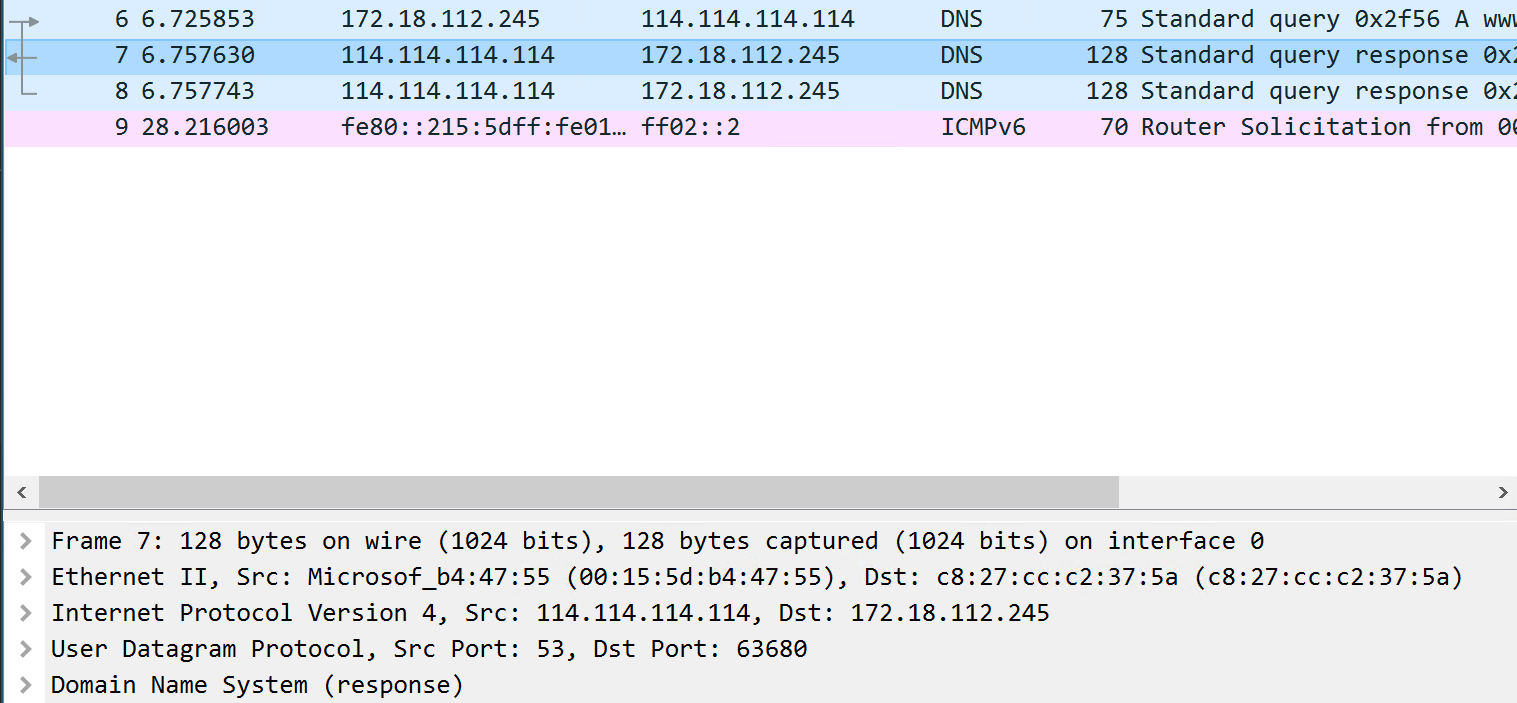
\includegraphics[width=0.8\linewidth]{assets/pic_udp.png}
      \caption{UDP stream of query by UDP.}
      \label{fig:pic_udp}
    \end{figure}
    3 UDP packets(datagrams?) are captured in this stream, port 63680 is used.
    \item The messages(DNS results) are exactly the same. The only difference between them are length, port and header.
  \end{itemize}
\end{itemize}

\newpage

\section*{Problem 3}

{\bf Description}

\begin{itemize}
  \item Function:
  \begin{itemize}
    \item Listen and accept DNS queries. Support common query types: A, AAAA, CNAME, TXT, NS, MX
    EDNS implementation is not required.
    \item Forward query to a upstream DNS resolver (or a public DNS server).
    \item Check out the response and send response to your clients.
    \item Maintain a cache of DNS query-response of all results.
  \end{itemize}
  \item Test method:
  \begin{itemize}
    \item using dig sending query to your resolver
  \end{itemize}
\end{itemize}

{\bf Solution}

See 5.3.zip/dns\_resolver.py. Serve on 127.0.0.1 and port 5300
\end{document}
